\documentclass[11pt]{beamer}

\usetheme{Warsaw}
%\addtobeamertemplate{navigation symbols}{}{%
%    \usebeamerfont{footline}%
%    \usebeamercolor[fg]{footline}%
%    \hspace{1em}%
%    \insertframenumber/\inserttotalframenumber
%}

\beamertemplatenavigationsymbolsempty

\setbeamertemplate{footline}
{
  \leavevmode%
  \hbox{%
  \begin{beamercolorbox}[wd=.333333\paperwidth,ht=2.25ex,dp=1ex,center]{author in head/foot}%
    \usebeamerfont{author in head/foot}\insertinstitute
  \end{beamercolorbox}%
  \begin{beamercolorbox}[wd=.333333\paperwidth,ht=2.25ex,dp=1ex,center]{title in head/foot}%
    \usebeamerfont{title in head/foot}\insertsubsection
  \end{beamercolorbox}%
  \begin{beamercolorbox}[wd=.333333\paperwidth,ht=2.25ex,dp=1ex,right]{date in head/foot}%
    \usebeamerfont{date in head/foot}\insertshortdate{}\hspace*{2em}
    \insertframenumber{} / \inserttotalframenumber\hspace*{2ex} 
  \end{beamercolorbox}}%
  \vskip0pt%
}
\usefonttheme[onlymath]{serif}

\usepackage{color}
\usepackage{xcolor}
\usepackage{tikz}
\usepackage{amsmath}
\usepackage{amssymb}
\usepackage{amsthm}
\usepackage{amsfonts}
\usepackage{graphicx}
\usepackage{mathtools}
\usepackage{wrapfig}
\usepackage{multirow}
\usepackage{comment}
\usepackage{natbib}
\usepackage{appendix}
\usepackage[utf8]{inputenc}
\usepackage{floatrow}
\usepackage{newfloat}
\usepackage{subcaption}
\usepackage{bm}

\usetikzlibrary{calc}
\usetikzlibrary{fit}
\usetikzlibrary{shapes.misc,calc, positioning, hobby, backgrounds}


%\DeclarePairedDelimiter{\floor}{\lfloor}{\rightfloor}
%\DeclarePairedDelimiter{\ceil}{\lceil}{\rceil}

\newcommand{\halflength}{\ensuremath{\floor{\frac{m}{2}}}}
\newcommand{\floor}[1]{\left \lfloor #1 \right \rfloor}
\newcommand{\ceil}[1]{\left \lceil #1 \right \rceil}

\newcommand{\oneline}[1]{\resizebox{\dimexpr\paperwidth - 3ex}{!}{#1}}

\DeclareFloatingEnvironment[fileext=los,
    listname={List of Example Figures},
    name=Example Figure,
    placement=tbhp,
    within=section,]{examplefigure}

\author{Thomas Lowbridge}
\title{Patrolling Games}
%\setbeamercovered{transparent} 
%\setbeamertemplate{navigation symbols}{} 
%\logo{} 
\institute{University Of Nottingham} 
%\date{} 
%\subject{} 
\begin{document}

\begin{frame}
\titlepage
\end{frame}

%\begin{frame}
%\tableofcontents
%\end{frame}

\begin{frame}{Introduction to Patrolling Games}
A Patrolling game, $G=G(Q,T,m)$ is made of 3 major components
\begin{itemize}
\item A Graph, $Q=(N,E)$, made of nodes, $N$ ($|N|=n$), and a set of edges, $E$.
\item A time horizon parameter, $T$ (with set $\mathcal{T}=\{0,1,...,T-1\}$).
\item An attack time parameter, $m$.
\end{itemize}

The game involves two players, the patroller and the attacker.
\begin{itemize}
\item The patroller's strategy is a walk (with waiting) on the graph, $W:\mathcal{T} \rightarrow  N$ .
\item The attacker's strategy is a node, $i$ and starting time, $\tau$ .
\end{itemize} 
The strategies are collected into the sets, $\mathcal{W}$ and $\mathcal{A}$ , for the patroller and attacker respectively, with some arbitrary labelling inside the set to form strategies $W_{i}$ and $A_{j}$.

\end{frame}

\begin{frame}{Payoffs}
The game is formulated as win-lose (a zero-sum game) with a payoff for the patroller of
\begin{align*}
P(W,(i,\tau))=\left\{ \begin{array}{l}
1 \text{  if  } i \in \left\{ W(\tau),W(\tau+1),...,W(\tau+m-1) \right\} ,\\
0 \text{  if  } i \notin \left\{ W(\tau),W(\tau+1),...,W(\tau+m-1) \right\} .\\
\end{array}\right.
\end{align*}
With a pure payoff matrix $\mathcal{P}=(P(W_{i},A_{j}))_{i \in \{ 1,...,|\mathcal{W}| \}, j \in \{ 1,...,|\mathcal{A}| \}}$
\end{frame}

\begin{frame}{Example of a game}
The game played on $Q$ as below with $m=3$ and $T=7$

\begin{center}
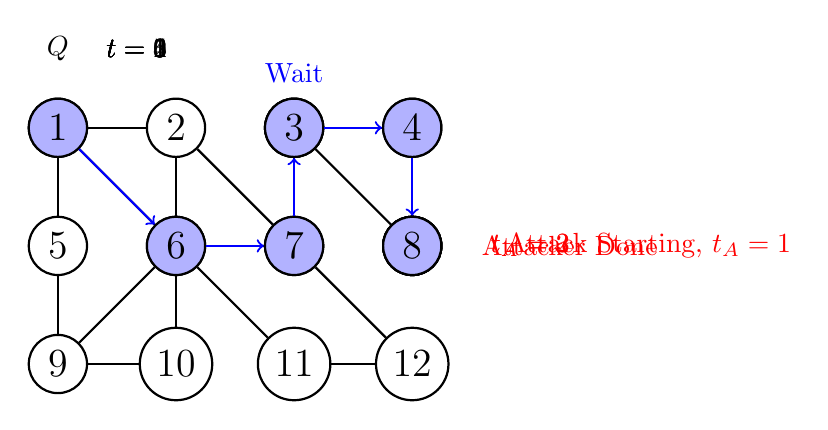
\begin{tikzpicture}[-,auto,node distance=1.5cm,
                    thick,main node/.style={circle,fill=white,draw,font=\sffamily\Large\bfseries}]

  \node[main node] (1) {$1$};
  \node[main node] (2) [right of=1] {$2$};
  \node[main node] (3) [right of=2]  {$3$};
  \node[main node] (4) [right of=3]  {$4$};
  \node[main node] (5) [below of=1]  {$5$};
  \node[main node] (6) [below of=2]  {$6$};
  \node[main node] (7) [below of=3]  {$7$};
  \node[main node] (8) [below of=4]  {$8$};
  \node[main node] (9) [below of=5]  {$9$};
  \node[main node] (10) [below of=6]  {$10$};
  \node[main node] (11) [below of=7] {$11$};
  \node[main node] (12) [below of=8] {$12$}; 

  \path[every node/.style={font=\sffamily}]
    (1) edge (2)
    (1) edge (5)
    (1) edge (6)
    (2) edge (6)
    (2) edge (7)
    (3) edge (7)
    (3) edge (4)
    (3) edge (8)
    (4) edge (8)
    (5) edge (9)
    (6) edge (7)
    (6) edge (10)
    (6) edge (11)
    (6) edge (9)
    (7) edge (12)
    (9) edge (10)
    (11) edge (12)
    ;

 \node (GraphLabel) [shift={(0,1)}] at (1) {$Q$}; 

%Slide 2 (first animation)
  \visible<2>{
  \node (TimeLabel) [shift={(1,1)}] at (1) {$t=0$};
  \node[main node,fill=blue!30] (1) at (1) {$1$};
  \path[->,color=blue] (1) edge (6); 
    }
%Slide 3
  \visible<3>{
  \node (TimeLabel) [shift={(1,1)}] at (1) {$t=1$};
  \node[main node,fill=blue!30] (6) at (6) {$6$};
  \path[->,color=blue] (6) edge (7); 
    }
%Slide 4
  \visible<4>{
  \node (TimeLabel) [shift={(1,1)}] at (1) {$t=2$};
  \node[main node,fill=blue!30] (7) at (7) {$7$};
  \path[->,color=blue] (7) edge (3);
  
  \node[main node,fill=red!30] (8) at (8) {$8$};
  \node[color=red] (Attacktimelabel) [shift={(3,0)}] at (8) {Attack Starting, $t_{A}=1$};
    }
%Slide 5
  \visible<5>{
  \node (TimeLabel) [shift={(1,1)}] at (1) {$t=3$};
  \node[main node,fill=blue!30] (3) at (3) {$3$};
  \node[color=blue] (WaitingLabel) [shift={(0,0.7)}] at (3) {Wait};
  
  \node[main node,fill=red!30] (8) at (8) {$8$};
  \node[color=red] (Attacktimelabel) [shift={(1.5,0)}] at (8) {$t_{A}=2$}; 
    }
%Slide 6
  \visible<6>{
  \node (TimeLabel) [shift={(1,1)}] at (1) {$t=4$};
  \node[main node,fill=blue!30] (3) at (3) {$3$};
  \path[->,color=blue] (3) edge (4);
  
  \node[main node,fill=red!30] (8) at (8) {$8$};  
  \node[color=red] (Attacktimelabel) [shift={(1.5,0)}] at (8) {$t_{A}=3$};
    }
%Slide 7
  \visible<7>{
  \node (TimeLabel) [shift={(1,1)}] at (1) {$t=5$};
  \node[main node,fill=blue!30] (4) at (4) {$4$};
  \path[->,color=blue] (4) edge (8); 
  
  \node[color=red] (Attacktimelabel) [shift={(2,0)}] at (8) {Attacker Done};
    }    
%Slide 8
  \visible<8>{
  \node (TimeLabel) [shift={(1,1)}] at (1) {$t=6$};
  \node[main node,fill=blue!30] (8) at (8) {$8$}; 
    }                 
\end{tikzpicture}

\end{center}
\only<1>{
\begin{itemize}
\item[\textcolor{blue}{Patroller:}] \textcolor{blue}{ $W(0)=1$ , $W(1)=6$ , $W(2)= 7$ , $W(3)=3$ , $W(4)=3$ , $W(5)=4$ , $W(8)= 8$}
\item[\textcolor{red}{Attacker:}] \textcolor{red}{$(8,2)$}
\end{itemize}
}
\only<8>
{
The attacker fails to catch the patroller, therefore the patroller loses (and the attacker wins) meaning a payoff of $0$ for the patroller (and $-1$ for the attacker).
}
\end{frame}

\begin{frame}{Mixed games}
Both the patroller and attacker will play their pure(realised) strategies with certain probabilities, let $\bm{\pi}$ be a mixed strategy for the patroller and let $\bm{\phi}$ be a mixed strategy for the attacker. We collect these into the sets $\Pi$ and $\Phi$ for the patroller and attacker respectively.

Then the payoff for the patroller of this mixed game becomes
\begin{align*}
P(\bm{\pi} ,\bm{\phi})=\sum\limits_{i=1}^{|\mathcal{W}|} \sum\limits_{j=1}^{|\mathcal{I}|} \mathcal{P}_{i,j} \bm{\pi} _{i} \bm{\phi}_{j}
=\bm{\pi} \mathcal{P} \bm{\phi}
\end{align*}

By using the pure payoff as $1$ when capture occurs and $0$ otherwise, the mixed payoff is equivalent to the probability of capture.
\end{frame}

\begin{frame}{Equilibrium and Value}
\begin{block}{Mixed Nash equilibrium}
A choice of $\bm{\pi}^*$ and $\bm{\phi}^*$ is said to be in \textit{Nash equilibrium} if 
\begin{align*}
P(\bm{\pi}^*,\bm{\phi}^*) \geq P(\bm{\pi},\bm{\phi}^*) \quad \forall \bm{\pi} \in \Pi , \\
P(\bm{\pi}^*,\bm{\phi}^*) \geq P(\bm{\pi}^*,\bm{\phi}) \quad \forall \bm{\phi} \in \Phi .
\end{align*}
\end{block}
There will only be one Nash equilibrium, unless the patroller can guarantee capture.

We do this by searching for the games value, $$V(G) \equiv \max\limits_{\bm{\pi} \in \Pi} \min\limits_{\bm{\phi} \in \Phi} P(\bm{\pi},\bm{\phi})=\min\limits_{\bm{\phi} \in \Phi} \max\limits_{\bm{\pi} \in \Pi} P(\bm{\pi},\bm{\phi})$$
This is done by achieving both upper and lower bounds on the value of the game.
\end{frame}

\begin{frame}{Solved graphs:Hamiltonian}

\begin{block}{Hamiltonian graphs}
A Hamiltonian graph has the value $V=\frac{m}{n}$
\end{block}

\end{frame}

\begin{frame}{Solved graphs:Bipartite}
\begin{block}{Bipartite graph}
A bipartite graph with no-adjacency partition into sets $A$ and $B$ has the value $V=\frac{m}{2(\max(|A|,|B|))}$
\end{block}
\end{frame}

\begin{frame}{Solved graphs:Star}
\begin{block}{Star graph}
The star $S_{n} \equiv K_{1,n}$ so has the value $V=\frac{m}{2n}$
\end{block}
\end{frame}

\begin{frame}{Solved graphs:Line}
\begin{block}{Line graph}
The line graph, $L_{n}$ made of $n$ nodes has a value dependent on $(n,m)$
\begin{enumerate}
\item If $m > 2(n-1)$ then $V=1$.
\item If $n-1 \leq m \leq 2(n-1)$ then $V=\frac{m}{2(n-1)}$
\item If $m=2 , n\geq 3$ then $V=\frac{1}{\ceil{\frac{n}{2}}}$
\item If $m=n-1 \text{ or } m=n-2  \text{ and } m=2k \text{ for some } k \geq 2 $ then $V=\frac{1}{2}$
\item If $m \leq n-3 \text{ or } m=n-2 \text{ and } m=2k+1 \text{ for some } k \geq 1$ then $V=\frac{m}{m+n-1}$
\end{enumerate}
\end{block}
\end{frame}



\end{document}